%Doc5
\chapter{Análisis}
\section{Caso de uso}
%Usar la página yuml.me
%Poner una "entidad o muñequito" por cada .h que hay la carpeta
%Reconocer celda, girar, moverse

%Código para el yuml.me:
%[Robot]-(Salir del laberinto)
%(Salir del laberinto)>(Robot.ino)
%(Robot.ino)<(Robot.hpp)
%(Robot.hpp)<(sInfrarrojos.hpp)
%(Robot.hpp)<(sUltrasonidos.hpp)
%(Robot.hpp)<(sCNY.hpp)
%(Robot.hpp)<(Motor.hpp)
%(Robot.hpp)<(Celda.hpp)
%(Robot.ino)>(StandardCplusplus)

Tenemos un operador, el robot, que necesita salir del laberinto. Para ello, utiliza el archivo \hyperlink{laberinto}{\texttt{Robot.ino}}, que incluye \hyperlink{StandardCplusplus}{\texttt{StandardCplusplus}} y extiende de \hyperlink{Robot}{\texttt{Robot.hpp}}, que a su vez, extiende de las librerías usadas para la implementación del código:
\begin{itemize}
	\item \hyperlink{Celda}{\textbf{\texttt{Celda.hpp:}}} De esta librería se extiende la implementación de las casillas y el manejo de las mismas.
	\item \hyperlink{Motor}{\textbf{\texttt{Motor.hpp:}}} De esta librería se extiende el control sobre los motores.
	\item \hyperlink{sCNY}{\textbf{\texttt{sCNY.hpp:}}} De esta librería se extiende el control de los sensores CNY.
	\item \hyperlink{sUltrasonidos}{\textbf{\texttt{sUltrasonidos.hpp:}}} De esta librería se extiende el control del sensor de ultrasonidos delantero.
	\item \hyperlink{sInfrarrojos}{\textbf{\texttt{sInfrarrojos.hpp:}}} De esta librería se extiende el control de los sensores de infrarrojos laterales.
\end{itemize}

\begin{center}
	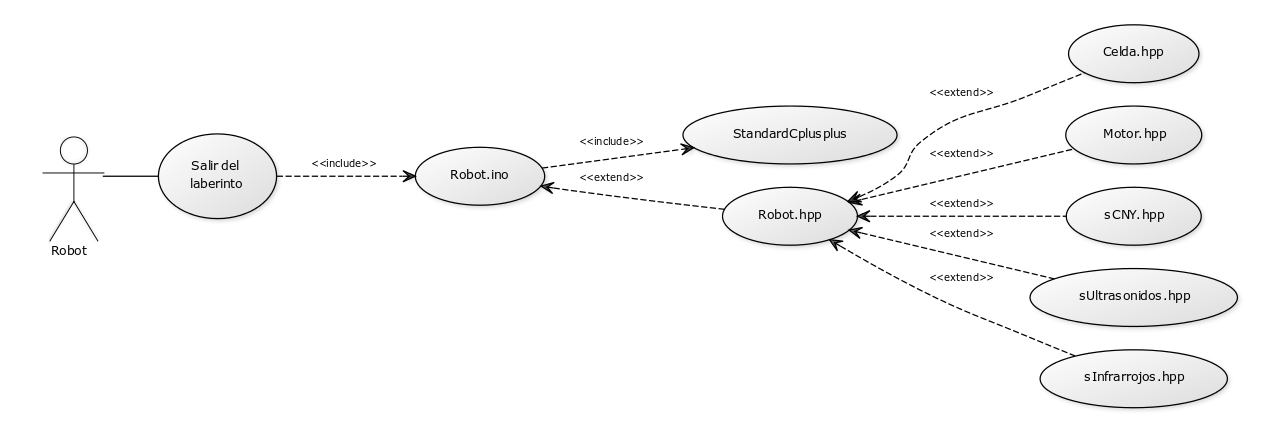
\includegraphics[scale=0.375]{CasoUso.png}
\end{center}
\newpage
\section{Diagrama de flujo}
%Utilizar draw.io o alguna similar
En el siguiente diagrama de flujo se ilustra el algoritmo que se ha implementado para intentar salir del laberinto.\\

\begin{center}
	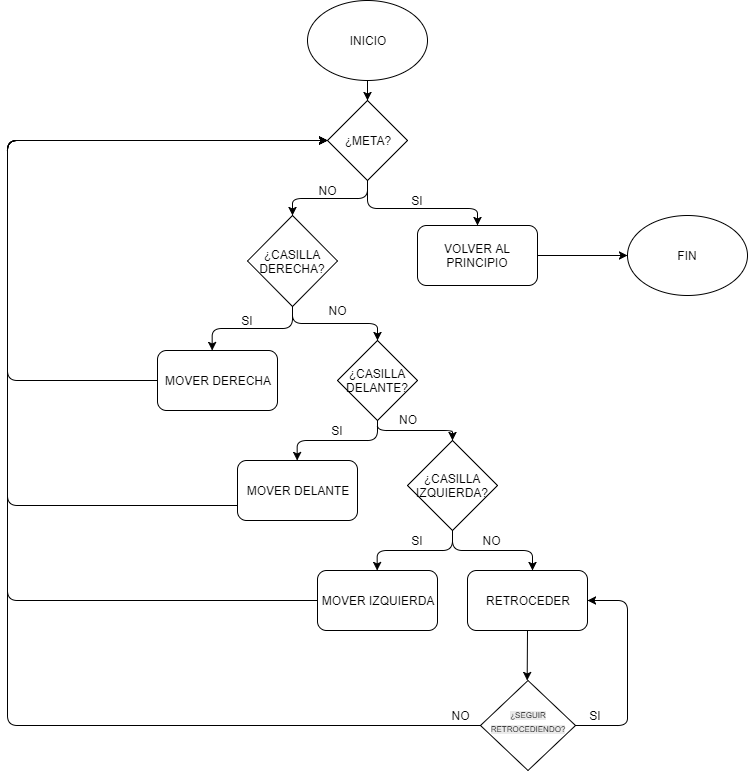
\includegraphics[scale=0.65]{DiagramaFlujo.png}
\end{center}
